\documentclass[../main.tex]{subfiles}
%!TEX root = ./analysisEnvelope.tex
\graphicspath {{../}}

\begin{document}
	
\subsection{Envelope Analysis} \label{envelopeAnalysis}
The envelope in this report is for reference only as Dr. Lateigne has made it clear he intends to design it. The model produced in Solidworks is generated based on the Graphic User Interface (GUI) based on the airship radius and total airship length (based on geometric relations with section length) seen in Figure ref{fig:envelopeDimensions}. The 10$^{\circ}$ was arbitrarily chosen as it looks more like a standard airship than other iterations. The fineness ratio is a relation of the diameter of the airship divided by the total length. Considering the airship travels at speeds well below the speed of sound, a low fineness ratio is expected. The envelope is expected to be deformed slightly by the thruster arms and thruster assembly, in order to have a significant contact area between them and the envelope.

	\begin{figure}[H]
	\centering
	\caption{Envelope Dimensions}
	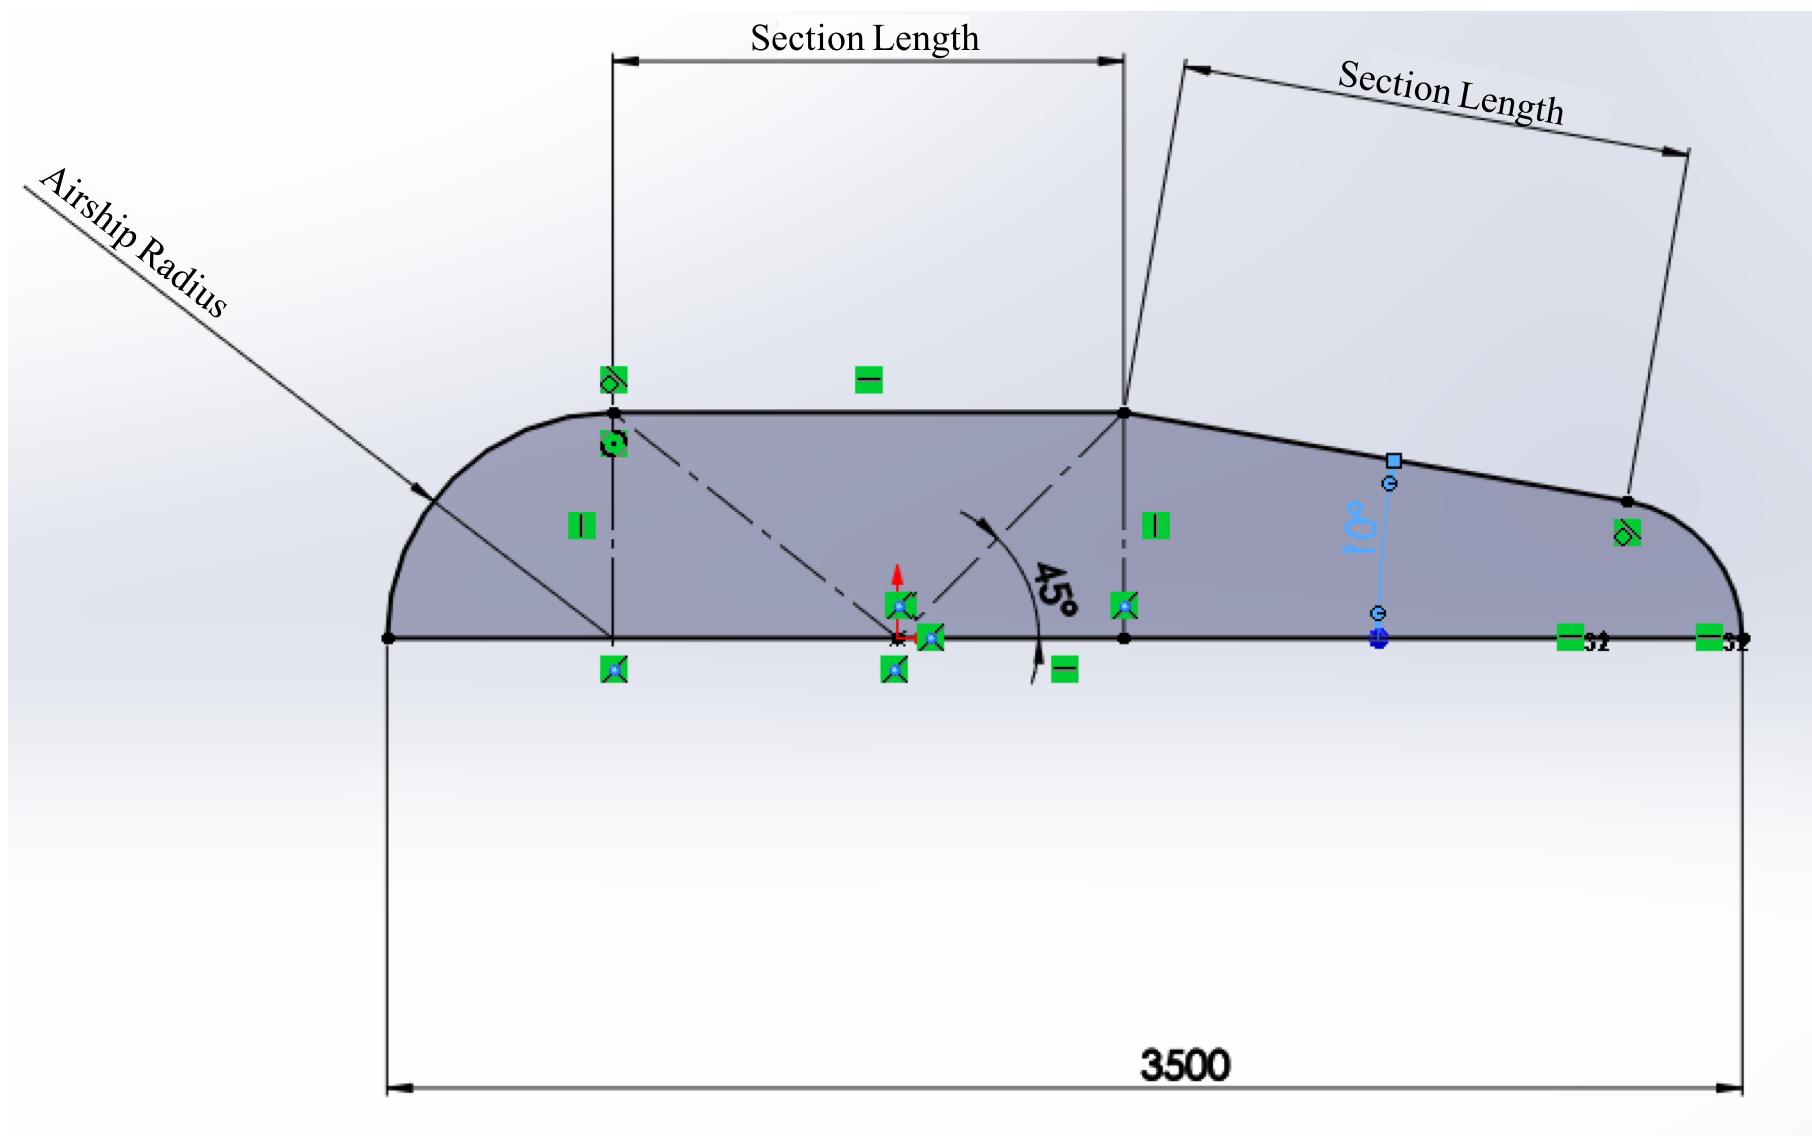
\includegraphics[width=.7\linewidth]{img/design/envelopeDimensions.png}
	\caption{Envelope Dimensions}
	\label{fig:envelopeDimensions}
\end{figure}
\end{document}